\chapter[Lens models]{Lens models}
\label{chap:lens_models}

This chapter delves into the intricate process of lens modeling, a pivotal technique for interpreting gravitational lensing observations. Gravitational lens models can be separated into two main categories: point-mass lenses (\ie \emph{microlenses}) and extended lenses, each possessing distinctive characteristics.
Microlensing refers to the lensing effect caused by objects with relatively small masses, such as stars or planets, acting as lenses. Unlike their more massive counterparts, microlenses do not produce multiple discernible images of the background source. Instead, they induce magnification variations over time as the lens moves relative to the observer and the source. 
Transitioning to a grander scale, extended lenses involve massive structures like galaxies and galaxy clusters, capable of producing multiple, resolvable images of background sources. 

% *************************************************************
%%%%% SECTION 3.1: MICROLENSES %%%%%
\section{Microlenses}
\label{sec:microlenses}

This section is devoted to exploring the phenomenon of microlensing, which refers to the lensing effects caused by objects of relatively small mass in the universe, such as planets, stars, star clusters, and other compact objects located within the Milky Way or distant galaxies. Typically, these microlenses are considered, in a first-order approximation, to be point-masses or collections of point-masses.


%%%%%%%%%%%%%%%%%%%%%%%%%%%%%%%%%%%%%%%%%%%%%%%%%%%%%%%
%%%%% Deflection angle and lensing potential %%%%%
%%%%%%%%%%%%%%%%%%%%%%%%%%%%%%%%%%%%%%%%%%%%%%%%%%%%%%%
\subsection{Deflection angle and lensing potential}
\label{subsec:angle_potential}
As already derived with \cref{eq:2.5}, by setting the lens position as the center of the reference frame and using the relation $\x = D_L \t$, the deflection angle for a point mass lens can be written as
\be
\label{eq:3.1}
\va{\a} (\va{\t}) = \frac{D_{LS}}{D_S} \hat{\va{\a}} (\va{\t}) = \frac{D_{LS}}{D_S} \frac{4 G M}{c^2 D_L} \frac{\va{\t}}{|\va{\t}|^2} \,.
\ee

Given that $\va{\a} (\va{\t}) = \va{\nabla} \hat{\P} (\va{\t})$, the lensing potential of the point mass lens is
\be
\label{eq:3.2}
\hat{\P} (\va{\t}) = \frac{4 G M}{c^2} \frac{D_{LS}}{D_L D_S} \ln{|\va{\t}|} \,.
\ee


%%%%%%%%%%%%%%%%%%%%%%%%%%%%%%%%%%%%%%%%%%%%%%%%%%%%%%%
%%%%% Lens equation and multiple images %%%%%
%%%%%%%%%%%%%%%%%%%%%%%%%%%%%%%%%%%%%%%%%%%%%%%%%%%%%%%
\subsection{Lens equation and multiple images}
\label{subsec:lenseq_images}
Given the deflection angle of \cref{eq:3.1}, the lens equation becomes
\be
\label{eq:3.3}
\b = \t - \frac{4 G M}{c^2 \t} \frac{D_{LS}}{D_L D_S} \,,
\ee
where the vector signs can be omitted due to the fact that the vector $\hat{\va{\a}}$ always points away from the lens.

As already anticipated in \cref{sec:lens_equation}, the lens equation can be written in a more concise way by introducing a scale radius $\t_E$, \ie the \emph{Einstein radius} defined in \cref{eq:2.30}, and setting $y = \b / \t_E$ and $x = \t / \t_E$, results:
\be
\label{eq:3.4}
\b = \t - \frac{\t_E^2}{\t} \quad \Rightarrow \quad y = x - \frac{1}{x} \,.
\ee
This equation is quadratic in $\t$ (or $x$) and has two solutions:
\be
\label{eq:3.5}
x_\pm = \frac{y \pm \sqrt{y^2 + 4}}{2} \,,
\ee
which means that there always exist two images for a given source position.

\begin{figure}
    \centering
    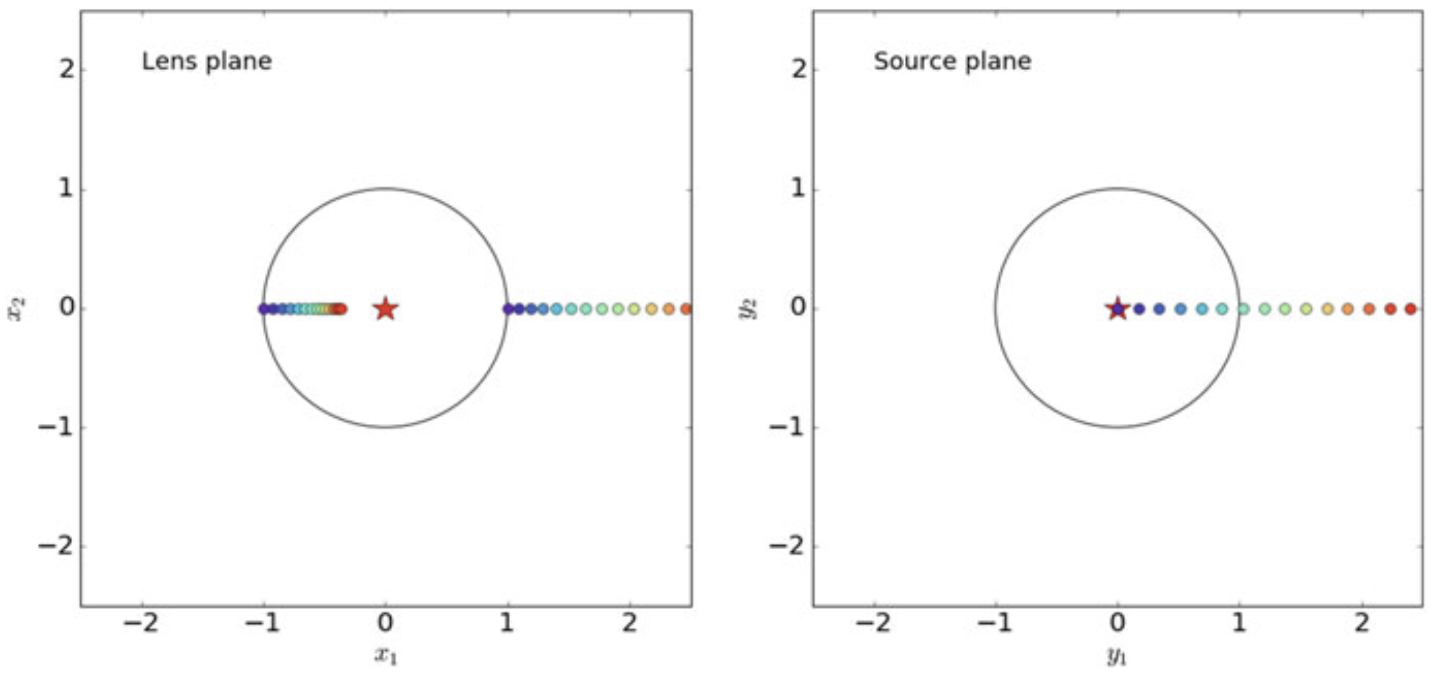
\includegraphics[width=\linewidth, keepaspectratio]{img//chapter3/pointmass_solutions.png}
    \caption[Lens equation solutions for point-mass lens]{Solutions of the lens equation for a point-mass, with the lens represented by the star at the center. The Einstein ring is highlighted in black. In the right diagram, the locations of various sources are marked with colored circles. The images produced, as calculated using \cref{eq:3.5}, are displayed in the left diagram.\\\small{Credits: \cite{meneghetti_introduction_2021}.}}
    \label{fig:pointmass_solutions}
\end{figure}

In the right section of \cref{fig:pointmass_solutions}, some sources are arranged at varying angular distances from the lens, which is marked by a red star. Each source is represented by a unique color to facilitate the identification of its corresponding images in the left section. Each source generates two images: one positioned at $x_+ > 0$ and the other in the range of $-1 < x_- < 0$. These images appear on either side of the lens, with the $x_-$ image always lying within a circle of radius $x = 1$. This circle is equivalent to the image produced by a source directly behind the point lens at $y = 0$, resulting in a ring-shaped image with radius $\t_E$, the Einstein ring.
The size of the Einstein radius is typically
\be
\label{eq:3.6}
\t_E \approx \SI{1}{\arcsecond} \bp{\frac{M}{10^{12} M_\odot}}^{1/2} \bp{\frac{D}{\si{\giga\parsec}}}^{-1/2} \,,
\ee
where
\be
\label{eq:3.7}
D \equiv \dfrac{D_L D_S}{D_{LS}}
\ee
is the \emph{effective lensing distance}.

As the angular separation $y \rightarrow 0$, it is observed that $x_- \rightarrow 0$, whereas $x_+ \rightarrow y$. This indicates that when the angular distance between the lens and the source increases significantly, the source is unlensed. In theory, an image still exists at $x_- = 0$, but this central image has zero magnification.


%%%%%%%%%%%%%%%%%%%%%%%%%%%%%%%%%%%%%%%%%%%%%%%%%%%%%%%
%%%%% Critical lines, caustics and magnification %%%%%
%%%%%%%%%%%%%%%%%%%%%%%%%%%%%%%%%%%%%%%%%%%%%%%%%%%%%%%
\subsection{Critical lines, caustics and magnification}
\label{subsec:critlines_caustics}
The Jacobian determinant for a point-mass lens can be written as
\be
\label{eq:3.8}
\det A (x) = \frac{y}{x} \frac{\dd{y}}{\dd{x}} \,,
\ee
which means that the eigenvalues of the Jacobian matrix are
\begin{subequations}
\begin{align}
    \label{eq:3.9a}
    \l_t (x) & = \frac{y}{x} = \bp{1 - \frac{1}{x^2}} \,,
    \\
    \label{eq:3.9b}
    \l_r (x) & = \frac{\dd{y}}{\dd{x}} = \bp{1 + \frac{1}{x^2}} \,.
\end{align}
\end{subequations}

The second eigenvalue is never zero, and therefore the point-mass lens only has a tangential critical line, a circle with equation $x^2 = 1$, which represents the Einstein ring.
This line can be mapped onto the source plane to find the relative tangential caustic, resulting in a single point at $y = 0$.

Given that the magnification is the inverse of the Jacobian determinant
\be
\label{eq:3.10}
\m (x) = \bp{1 - \frac{1}{x^4}}^{-1} \,,
\ee
which can also be written as a function of the source position
\be
\label{eq:3.11}
\m_\pm (y) = \frac{x}{y} \frac{\dd{x}}{\dd{y}} = \frac{1}{2} \bp{1 \pm \frac{y^2 + 2}{y \sqrt{y^2 + 4}}} \,,
\ee
the magnifications of the two images always have the same signs of $x_\pm$ and therefore different parity.

The total source magnification will then be:
\be
\label{eq:3.12}
\m (y) = \m_+ (y)  + |\m_- (y)| = \frac{y^2 + 2}{y \sqrt{y^2 + 4}} \,,
\ee
while the sum of the signed magnifications is always $\m = 1$.

Furthermore, it can be shown through series expansion that, for large $y$,
\be
\label{eq:3.13}
\lim_{y\to\infty} \left| \frac{\m_+}{\m_-} \right| \propto y^4 \,.
\ee
This means that the magnification rapidly becomes negligible outside the Einstein ring and has a very simple form well inside it. Hence, deviations from simple point-lens microlensing can usually be easily spotted.


%%%%%%%%%%%%%%%%%%%%%%%%%%%%%%%%%%%%%%%%%%%%%%%%%%%%%%%
%%%%% Microlensing light-curve %%%%%
%%%%%%%%%%%%%%%%%%%%%%%%%%%%%%%%%%%%%%%%%%%%%%%%%%%%%%%
\subsection{Microlensing light-curve}
\label{subsec:micro_lc}
The Einstein radius of a typical lens indicates the scale of image separation observed in microlensing events. For a star with the mass of the Sun located within the Milky Way, the separation is approximately of the order of milliarcseconds, a measurement that is beyond the detection capabilities of current instruments. However, stars move around the Galactic center (and have an additional random velocity component with respect to one another). The relative velocities are such that the time scale of the relative change of lens and source positions is of order of weeks or shorter. Therefore, this motion introduces a temporal component in the lensing geometry, causing the distance between the lens and the source, and thus the magnification, to vary measurably as a function of time, accordingly to \cref{eq:3.12}. In general, a source with intrinsic flux $F_s$ will appear to have flux $F (t) = \m (t) F_s$. 
\newpage
The \emph{microlensing light-curve} describes the temporal behavior of the magnification, dictated by the relative motion of the lens across the observer-source line of sight.

\begin{figure}
    \centering
    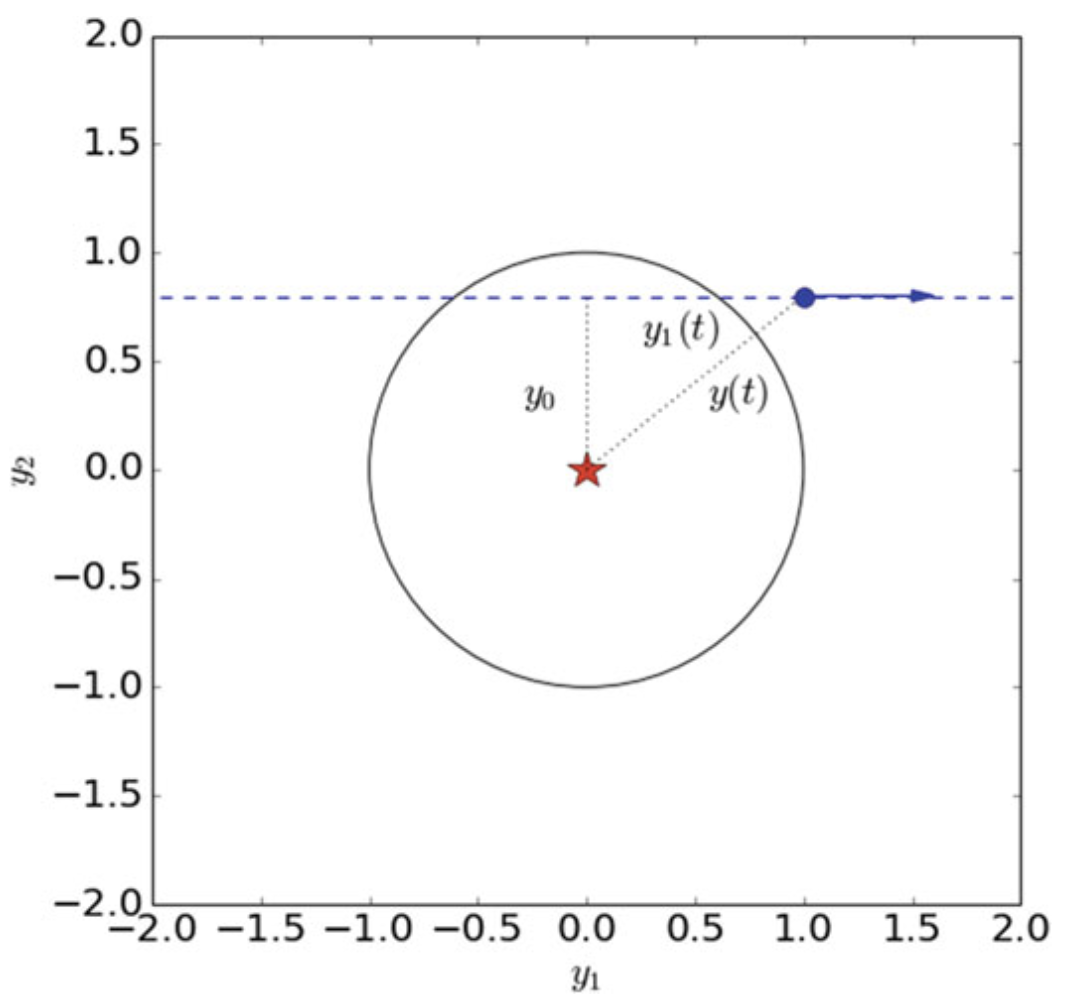
\includegraphics[width=0.61\linewidth, keepaspectratio]{img//chapter3/lens_source_trajectory.png}
    \caption[Lens position and source trajectory in a microlensing event]{Illustration of the lens position and source trajectory. The dimensionless impact parameter is $y_0$, $y_1 (t)$ indicates the dimensionless distance of the source from its closest point to the lens, and $y (t)$ is the dimensionless distance between the lens and source.\\\small{Credits: \cite{meneghetti_introduction_2021}.}}
    \label{fig:lens_source_trajectory}
\end{figure}

As shown in \cref{fig:lens_source_trajectory}, assuming a straight line can approximate the path of the source relative to the lens, the former moving with transverse velocity $v$ and reaching the minimum dimensionless distance $y_0$ (\ie the \emph{impact parameter} of the source), from the lens at time $t_0$, the dimensionless distance of the source from $y_0$ can be written
\be
\label{eq:3.14}
y_1 (t) = \frac{v (t - t_0)}{D_L \t_E} \,.
\ee

Since magnification significantly deviates from unity only for sources with $|y| \lesssim 1$, the characteristic timescale of the microlensing event is given by
\be
\label{eq:3.15}
t_E = \frac{D_L \t_E}{v} \,,
\ee
which is known as the \emph{Einstein crossing time}. Stellar lenses in the Milky Way are associated with typical $t_E$ on the order of a month, and thus the changes in the observed brightness of the source they induce are referred to as microlensing ``events''.

Inserting \cref{eq:3.15} into \cref{eq:3.14}, the trajectory of the source can be represented by
\be
\label{eq:3.16}
y (t) = \sqrt{y_0^2 + y_1^2 (t)} = \sqrt{y_0^2 + \frac{(t - t_0)^2}{t_E^2}}  \,.
\ee

The corresponding light-curve of the source, examples of which are shown in \cref{fig:light_curves}, is then obtained by combining \cref{eq:3.16,eq:3.12} and multiplying by the unlensed source flux
\be
\label{eq:3.17}
F (t) = \m (t) F_s = \frac{y (t)^2 + 2}{y (t) \sqrt{y (t)^2 + 4}} F_s  \,.
\ee

\begin{figure}
    \centering
    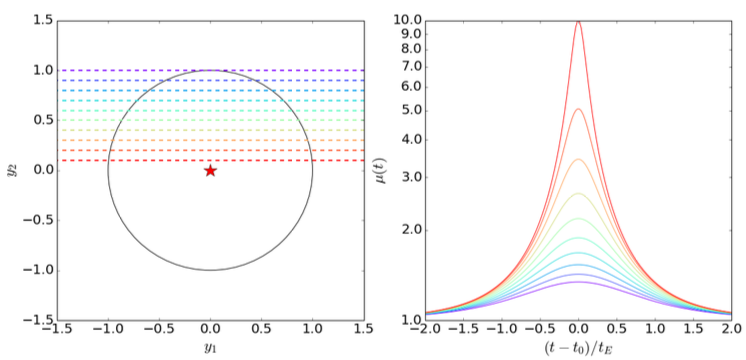
\includegraphics[width=\linewidth, keepaspectratio]{img//chapter3/light_curves.png}
    \caption[Microlensing light-curves for different impact parameters]{Left panel: some examples of source trajectory across the Einstein ring with different impact parameters $y_0$. Right panel: corresponding light-curves.\\\small{Credits: \cite{meneghetti_introduction_2021}.}}
    \label{fig:light_curves}
\end{figure}

The \emph{standard} microlensing light-curve of a simple point-source, point-lens system is thus described by four parameters: unlensed flux $F_s$, $t_0$, $y_0$ and $t_E$. Of these, $F_s$ can be measured in the absence of microlensing, $t_0$ and $y_0$ from the position and height of the light-curve peak, respectively. Only $t_E= D_L \t_E / v$ contains physical information about the lens system and determines the peak width, \ie the duration of the event. Assuming that the source distance can be determined from its properties (membership in a stellar system, spectral type and apparent magnitude), there are three physical parameters, lens mass $M$, lens distance $D_L$, and lens relative transverse velocity $v$, to determine from one observable: this is the so-called \emph{microlensing degeneracy}. 
Although the standard light-curve model is successful in numerous instances, there exist circumstances where some foundational assumptions of this model no longer hold. In such situations, it might be feasible to derive additional constraints that can partially lift the degeneracy. Non-standard light-curves, for instance, may occur when either the source or the lens are not point-like, or when the path of the source moving relative to the lens is not linear. Such instances often occur when either the lens or the source, or both, are part of binary systems.

% *************************************************************
%%%%% SECTION 3.2: EXTENDED LENSES %%%%%
\section{Extended lenses}
\label{sec:ext_lenses}
This section aims to introduce the main models used to represent extended gravitational lenses, such as massive galaxies and galaxy clusters. These cosmic structures, characterized by their complex, gravitationally bound mass distributions, are formidable gravitational lenses capable of producing striking lensing phenomena, including multiple images and gravitational arcs.

The analysis starts with circular, axially symmetric models and describes how different mass profiles affect lensing properties. Subsequently, deviations from circular symmetry are introduced through properties such as ellipticity and substructures. Finally, the impact of the environment surrounding the lenses is taken into account. The thin screen approximation is used throughout this description of analytical lens models.


%%%%%%%%%%%%%%%%%%%%%%%%%%%%%%%%%%%%%%%%%%%%%%%%%%%%%%%
%%%%% Axially symmetric profiles %%%%%
%%%%%%%%%%%%%%%%%%%%%%%%%%%%%%%%%%%%%%%%%%%%%%%%%%%%%%%
\subsection{Axially symmetric profiles}
\label{subsec:axially_profiles}
The most simple description of an extended lens is an axially symmetric profile. For such lenses, the potential is constant on circles centered on the lens center. This symmetry allows most equations to be simplified to a one-dimensional form.

The deflection angle is radially directed and its amplitude depends only on the distance from the lens center. Its expression is the same as that of the point-mass lens, with the only difference that now $M = M(\t)$ is the mass enclosed in a circle of radius $\t$. For this reason, introducing an arbitrary reference scale $\x_0$, the \emph{dimensionless mass} profile can be written as
\be
\label{eq:3.18}
m (x) = 2 \int_0^x x^\prime \k (x^\prime) \dd{x^\prime} = \frac{M (\x_0 x)}{\pi \x_0^2 \S_{cr}} \,, 
\ee
which leads to a deflection angle
\be
\label{eq:3.19}
\a (x) = \frac{2}{x} \int_0^x x^\prime \k (x^\prime) \dd{x^\prime} = \frac{m (x)}{x} \,.
\ee

Therefore, the lens equation is
\be
\label{eq:3.20}
y = x - \frac{m (x)}{x} \,.
\ee

Given that $\P^\prime (x) = \a (x)$, from \cref{eq:2.17} the convergence profile can be obtained:
\be
\label{eq:3.21}
\k (x) = \frac{1}{2} \bs{\a^\prime (x) + \frac{\a (x)}{x}} = \frac{m^\prime (x)}{2 x} \,.
\ee

Finally, introducing $\overline{\k} (x) = m (x) / x^2$ as the mean convergence within a circle of radius $x$, the shear vector results
\be
\label{eq:3.22}
\g (x) = \frac{1}{2} \left| \a^\prime (x) - \frac{\a (x)}{x} \right| = |\k (x) - \overline{\k} (x)| \,.
\ee

Using the precedent results and \cref{eq:2.24}, it is possible to compute the determinant of the lensing Jacobian
\be
\label{eq:3.23}
\det A (x) = \frac{y}{x} \frac{\dd{y}}{\dd{x}} = [1 - \k (x) - \g (x)] [1 - \k (x) + \g (x)] \,,
\ee
and the correspondent magnification profile $\m (x) = [\det A (x)]^{-1}$.

As described in \cref{sec:lens_equation}, the set of points that satisfies $\det A (x) = 0$ represents the critical lines of the lens. For an axially symmetric lens these are circles, whose radii can be found by solving the equations
\begin{subequations}
\begin{align}
    \label{eq:3.24a}
    \l_t (x) & = 0 \quad \Rightarrow \quad \k (x) + \g (x) = 1 \,,
    \\
    \label{eq:3.24b}
    \l_r (x) & = 0 \quad \Rightarrow \quad \k (x) - \g (x) = 1 \,,
\end{align}
\end{subequations}
which define the \emph{tangential critical line} and the \emph{radial critical line}, respectively.

Through the lens equation, it can be seen that all the points along the tangential critical line are mapped to the point $y = 0$ on the source plane: this type of lenses have point-like tangential caustics. Instead, the radial critical points are mapped onto a circular radial caustic on the source plane.


%%%%%%%%%%%%%%%%%%%%%%%%%%%%%%%%%%%%%%%%%%%%%%%%%%%%%%%
%%%%% Power-law profiles %%%%%
%%%%%%%%%%%%%%%%%%%%%%%%%%%%%%%%%%%%%%%%%%%%%%%%%%%%%%%
\subsection{Power-law profiles}
\label{subsec:power_law_profiles}
This class of lenses is characterized by a mass profile with a power-law form of the kind
\be
\label{eq:3.25}
m (x) = x^{3-n} \,,
\ee
where $n$ is a parameter that can assume any real value $>1$.

From the previous mass profile definition, all the other lensing properties can be derived:
\begin{equation}
\label{eq:3.26}
\begin{aligned}
    \k (x) & = \frac{m^\prime (x)}{2 x} = \frac{3 - n}{2} x^{1 - n} \,, \\[5pt]
    \a (x) & = \frac{m (x)}{x} = x^{2 - n} \,, \\[5pt]
    \g (x) & = \left| \frac{m^\prime}{2 x} - \frac{m (x)}{x^2} \right| = \frac{n - 1}{2} x^{1 - n} \,, \\[5pt]
    y & = x - x^{2-n} \,.
\end{aligned}
\end{equation}

In particular, given the value of the parameter $n$, it is possible to distinguish different scenarios.
\begin{itemize}
    \item \textbf{n = 1}: perfectly convergent lens with constant convergence and $y (x) = 0$, $\forall x$;
    
    \item \textbf{1 < n < 2}: mass and deflection angle profiles increase with $x$, while the convergence and shear profiles show a decrease. The tangential critical line forms a circle of radius $x_t = 1$, $\forall n$, and its corresponding caustic line is a single point at $y_t = 0$. On the other hand, the size of the radial critical line varies according to the value of $n$. As it increases, the radial critical line becomes smaller, whereas the size of the caustic line follows an increasing trend. In particular, for $n = 2$, the radial critical line is absent. For lenses that are axially symmetric, there are multiple methods to solve the lens equation, but the most effective approach is often referred to as the \emph{image diagram}, by which multiple image positions can be identified where the profile of the deflection angle intersects the lines $f(x) = x - y$.
    
    \Cref{fig:image_diagrams_1_2} demonstrates that the separation between images is influenced by the value of $n$: a higher value results in a more curved profile of the deflection angle, leading to a greater number of images that are closer together, and conversely, a lower $n$ leads to fewer images with larger separations. More precisely, these lenses produce three images if the source is inside the radial critical line (\ie $\,y < y_r$), otherwise they form a single image.
    
    \item \textbf{n = 2}: flat deflection angle profile, Singular Isothermal Sphere model (see \cref{subsec:sis});
    
    \item \textbf{n > 2}: deflection angle profile decreases with $x$ and has a singularity in $x = 0$. These lenses produce two images, one inside and one outside the Einstein radius (see \cref{fig:image_diagrams_2}). The radial eigenvalue is always non-zero, causing the absence of a radial critical line and ensuring that the radial magnification factor, $\m_r < 1$, always. This means that the images are consistently demagnified in the radial direction.
    
    It should be noted that for $n = 3$ the scenario corresponds to that of a point-mass lens.
\end{itemize}

\begin{figure}[h!]
    \centering
    \includegraphics[width=\linewidth, keepaspectratio]{img//chapter3/image_diagrams_1_2.png}
    \caption[Image diagrams for power-law lenses with $1<n<2$]{Image diagrams for different values of $1<n<2$. The solid curves show the function $\a (x)$, while the dashed lines represent the function $f (x) = x - y$, with varying $y$ value.}
    \label{fig:image_diagrams_1_2}
\end{figure}

\begin{figure}[h!]
    \centering
    \includegraphics[width=\linewidth, keepaspectratio]{img//chapter3/image_diagrams_2.png}
    \caption[Image diagrams for power-law lenses with $n>2$]{Image diagrams for different values of $n>2$. The solid curves show the function $\a (x)$, while the dashed lines represent the function $f (x) = x - y$, with varying $y$ value.}
    \label{fig:image_diagrams_2}
\end{figure}


%%%%%%%%%%%%%%%%%%%%%%%%%%%%%%%%%%%%%%%%%%%%%%%%%%%%%%%
%%%%% Singular Isothermal Sphere %%%%%
%%%%%%%%%%%%%%%%%%%%%%%%%%%%%%%%%%%%%%%%%%%%%%%%%%%%%%%
\subsection{Singular Isothermal Sphere}
\label{subsec:sis}
One of the simplest and most widely used models for axially symmetric lenses is the Singular Isothermal Sphere (SIS). The density profile is obtained by assuming that the matter constituting the lens acts like an ideal gas, contained within a spherically symmetric gravitational potential. This gas is presumed to be in states of thermal and hydrostatic equilibrium.

By projecting the three-dimensional density onto the lens plane, the surface mass density can be calculated
\be
\label{eq:3.27}
\S (\x) = \int_0^\infty \r (\x, z) \dd{z} = \frac{\s_v^2}{2 G \x} \,,
\ee
where $\x$ is the distance from the center of the lens and $\s_v$ represents the gas particle velocity dispersion (\ie the stars in a galaxy or the galaxies in a cluster).
Although this profile is not physical, having a singularity for $\x = 0$ and an infinite total mass, it reproduces very well the observed flat rotation curves of spiral galaxies for $0 \ll \x < \infty$.

Setting the length scale at $\x_0 = 4 \pi \bp{\frac{\s_v}{c}}^2 \frac{D_L D_{LS}}{D_S}$, it is possible to rewrite \cref{eq:3.27} in a dimensionless form and derive the convergence profile
\be
\label{eq:3.28}
\S (x) = \frac{\S_{cr}}{2 x} \quad \Rightarrow \quad \k (x) = \g (x) = \frac{1}{2 x} \,,
\ee
which shows that the SIS lens corresponds to a power-law lens with $n=2$.

From the convergence definition, the deflection angle and the lens equation can be obtained:
\begin{subequations}
\begin{align}
    \label{eq:3.29a}
    &\a (x) = \frac{x}{|x|} \,,
    \\
    \label{eq:3.29b}
    &y = x - \frac{x}{|x|} \,.
\end{align}
\end{subequations}

The solutions of the lens equation are dependent on the source position $y$, as it can be seen in the left panel of \cref{fig:image_diagrams_2}:
\begin{itemize}
    \item when $0 < y < 1$ there exist two solutions on opposite sides of the lens center; one is at $x_- = y - 1$ and one at $x_+ = y + 1$. Their angular separation is always $\D (\t_E) = 2 \t_E$;

    \item when $y > 1$ there is only one solution at $x_+ = y + 1$.
\end{itemize}

Therefore, the circle of radius $y = 1$ serves a similar function to that of the radial caustic for power-law lenses with $1 < n < 2$, delineating areas on the source plane that are associated with different image multiplicities. However, this circle does not qualify as caustic because $\a^\prime (x) = 0$, $\forall x$, indicating that $\l_r = 1$. Instead, the circle of radius $y_{cut} = 1$ is referred to as pseudo-caustic, known as the \emph{cut}. In addition, unlike ''normal" caustics, the number of images changes only by one when crossing the cut, instead of changing by two.

Given that $\l_r = 1$, the images are only magnified in the tangential direction, while the radial size of all the images remains unchanged. In particular, when the source is placed inside the cut, the magnifications can be expressed as:
\begin{subequations}
\begin{align}
    \label{eq:3.30a}
    \m_- (y) & = 1 - \frac{1}{y} \,,
    \\
    \label{eq:3.30b}
    \m_+ (y) & = 1 + \frac{1}{y} \,,
\end{align}
\end{subequations}
for the image inside and outside the Einstein ring respectively.

From \cref{eq:3.30a,eq:3.30b} can be seen that for $y \rightarrow 1$ the image $x_-$ becomes weaker and weaker until it disappears for $y = 1$. On the other hand, when $y \rightarrow \infty$ the source magnification tends to unity: sources at a large distance from the lens experience little to no magnification.

\Cref{fig:sis_extended} shows some examples of images produced by a SIS lens of an extended circular source, placed at different distances from the lens.

\begin{figure}
    \centering
    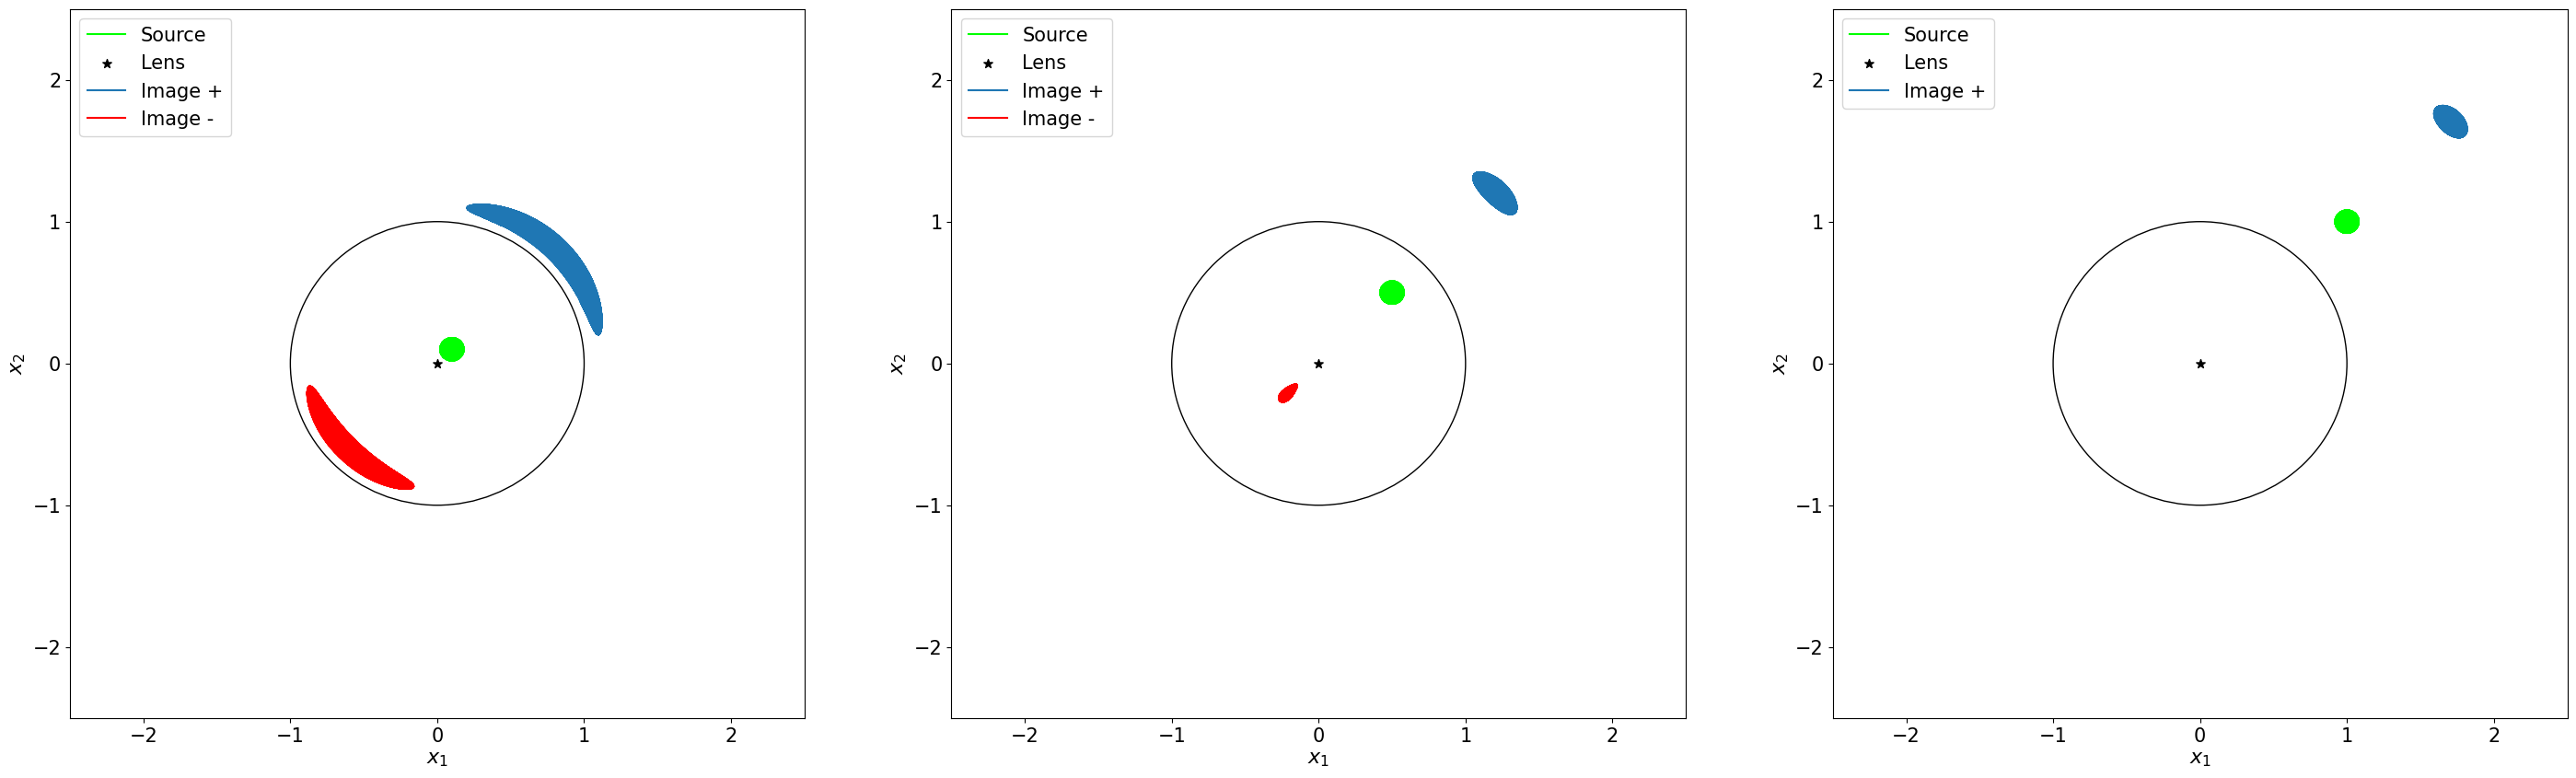
\includegraphics[width=\linewidth, keepaspectratio]{img//chapter3/sis_extended.png}
    \caption[Imaging of an extended source by a SIS lens]{Imaging of an extended source by a SIS lens. Each panel shows the images produced for different values of $y$. The black circle represents the tangential critical line of the lens, the Einstein ring.}
    \label{fig:sis_extended}
\end{figure}


%%%%%%%%%%%%%%%%%%%%%%%%%%%%%%%%%%%%%%%%%%%%%%%%%%%%%%%
%%%%% Non-singular Isothermal Sphere %%%%%
%%%%%%%%%%%%%%%%%%%%%%%%%%%%%%%%%%%%%%%%%%%%%%%%%%%%%%%
\subsection{Non-singular Isothermal Sphere}
\label{subsec:nis}
One way to solve the central singularity issue of the SIS lens is to introduce an additional parameter $\x_c$, describing a flat central core of the surface density profile \citep{kormann_isothermal_1994}:
\be
\label{3.31}
\S (\x) = \frac{\S_0}{\sqrt{1 + (\x / \x_c)^2}} \quad \mathrm{with} \quad \S_0 = \frac{\s_v^2}{2 G \x_c} \,,
\ee
where $\S_0$ represents the constant surface density for $\x \ll \x_c$.

By introducing the same scale length $\x_0$ defined in \cref{subsec:sis} and re-scaling both $\x$ and $\x_c$, the dimensionless relevant quantities for the Non-singular Isothermal Sphere (NIS) can be derived:
\begin{equation}
\label{eq:3.32}
\begin{aligned}
    &\k (x) = \frac{1}{2 \sqrt{x^2 + x_c^2}} \,, \\[5pt]
    &\m (x) = \sqrt{x^2 + x_c^2} - x_c \,, \\[5pt]
    &\a (x) = \sqrt{1 + \bp{\frac{x_c}{x}}^2} - \frac{x_c}{x} \,, \\[5pt]
    &y = x - \sqrt{1 + \bp{\frac{x_c}{x}}^2} - \frac{x_c}{x} \,.
\end{aligned}
\end{equation}

The lens equation above can be reduced to a third-order polynomial: the NIS lens can produce up to three images of a given source, with multiplicity depending on the value of $x_c$. It can be shown \citep{meneghetti_introduction_2021} that tangential and critical lines exist only for values of $x_c < 1/2$, \ie for $x_c > 1/2$ the lens is ``weak'' and cannot produce multiple images.
In particular, the tangential caustic is a point at $y_t = 0$, while the radii of the tangential critical line, the radial caustic and the radial critical line vary with $x_c$ as shown in \cref{fig:nis_radii}. 

\begin{figure}[b!]
    \centering
    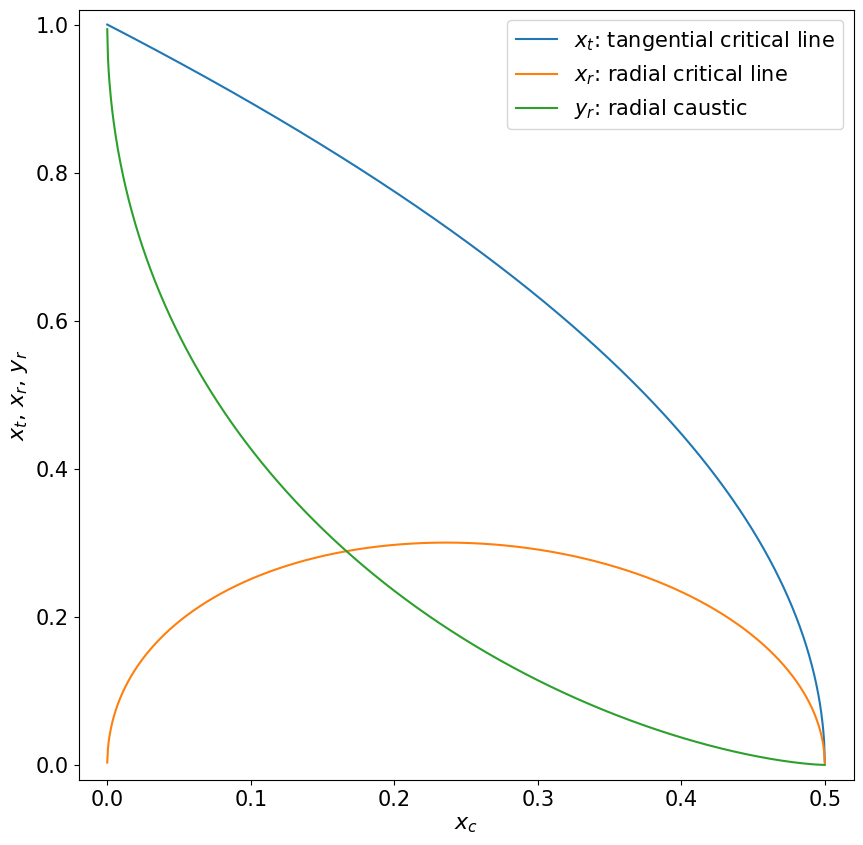
\includegraphics[width=0.65\linewidth]{img//chapter3/nis_radii.png}
    \caption[NIS caustic critical lines radii as a function of $x_c$]{NIS caustic critical lines radii as a function of $x_c$. For $x_c = 0$, $y_r = 1$, \ie the SIS cut.}
    \label{fig:nis_radii}
\end{figure}


%%%%%%%%%%%%%%%%%%%%%%%%%%%%%%%%%%%%%%%%%%%%%%%%%%%%%%%
%%%%% Singular Isothermal Ellipsoid %%%%%
%%%%%%%%%%%%%%%%%%%%%%%%%%%%%%%%%%%%%%%%%%%%%%%%%%%%%%%
\subsection{Singular Isothermal Ellipsoid}
\label{subsec:sie}
After investigating the impact of altering the slope of the density profile and the incorporation of a central core, it is possible to assess the influence of ellipticity on lens characteristics. Introducing ellipticity surely improves the representation of galaxies and their mass distributions. \cite{kormann_isothermal_1994} developed the Singular Isothermal Ellipsoid (SIE) model, which can be derived from the SIS model by substituting
\be
\label{eq:3.33}
\x \quad \Rightarrow \quad \sqrt{\x_1^2 + f^2 \x_2^2} \,,
\ee
where $0 < f \leq 1$ is the axis ratio of the ellipses that, in this scenario, define the iso-density contours of the mass profile.

Through this substitution, the surface density profile becomes
\be
\label{eq:3.34}
\S (\va{\x}) = \frac{\s_v^2}{2 G} \frac{\sqrt{f}}{\sqrt{\x_1^2 + f^2 \x_2^2}}  \,,
\ee
which, as already said, is constant on ellipses with minor axis $\x$ and major axis $\x / f$.

By choosing, once again, the same scale length $\x_0$ as for the SIS model, the convergence can be written as
\be
\label{eq:3.35}
\k (\vec{x}) = \frac{\sqrt{f}}{2 \sqrt{x_1^2 + f^2 x_2^2}}  \,,
\ee
or, using polar coordinates,
\be
\label{eq:3.36}
\k (x, \varphi) = \frac{\sqrt{f}}{2 x \D (\varphi)}  \,,
\ee
where
\be
\label{eq:3.37}
\D (\varphi) = \sqrt{\cos{(\varphi)}^2 + f^2 \sin{(\varphi)}^2}  \,.
\ee

By solving the Poisson equation, the lensing potential in polar coordinates can be obtained, and then, taking its gradient, it is possible to derive the deflection angle, which has two components, none of which depends on $x$:
\begin{equation}
\begin{aligned}
    \label{eq:3.38}
    \a_1 (\vec{x}) & = \sqrt{\frac{f}{1 - f^2}} \arcsinh \bp{\frac{\sqrt{1 - f^2}}{f} \cos{(\varphi)}} \,,
    \\
    \a_2 (\vec{x}) & = \sqrt{\frac{f}{1 - f^2}} \arcsin \bp{\sqrt{1 - f^2} \sin{(\varphi)}} \,.
\end{aligned}
\end{equation}

The shear components can be obtained from the derivatives of the deflection angle
\begin{equation}
\begin{aligned}
    \label{eq:3.39}
    \g_1 (\vec{x}) & = - \k (\vec{x}) \cos{(2 \varphi)} \,,
    \\
    \g_2 (\vec{x}) & = - \k (\vec{x}) \sin{(2 \varphi)} \,,
\end{aligned}
\end{equation}
and, as for the SIS model, $\g = \sqrt{\g_1^2 + \g_2^2} = \k$.

Finally, from the lensing Jacobian determinant, the two eigenvalue are
\begin{subequations}
\begin{align}
    \label{eq:3.40a}
    \l_t (\vec{x}) & = 1 - 2 \k (\vec{x}) \,,
    \\
    \label{eq:3.40b}
    \l_r (\vec{x}) & = 1 \,.
\end{align}
\end{subequations}

Similarly to the SIS lens, the SIE does not have a radial critical line. Instead, the tangential critical line is the ellipse defined by
\be
\label{eq:3.41}
\k (\vec{x}) = \frac{1}{2} \quad \Rightarrow \quad \vec{x}_t (\varphi) = \frac{\sqrt{f}}{\D (\varphi)} [\cos{(\varphi)}, \sin{(\varphi)}] \,.
\ee

As always, the points on the critical line can be mapped onto the source plane using the lens equation: introducing ellipticity to the lens disrupts its axial symmetry, leading to the transformation of the tangential caustic from a central point into an astroid-shaped caustic, featuring four cusps and four folds. As for the SIS, due to the singularity at the center of the lens, also for the SIE profile does not exist a radial critical line and, as a result, the multiple images region is not enclosed by the radial caustic, but by the cut, which is an ellipse.

The number of multiple images formed by this lens is influenced by the positioning of the cut and caustic lines. In particular, for large ellipticities (small values of $f$, in particular $f < f_0 = 0.3942$), the tangential caustic extends outside the cut, as shown in \cref{fig:naked_cusps}. The cusps that are not contained within the cut are called \emph{naked}.

\begin{figure}
    \centering
    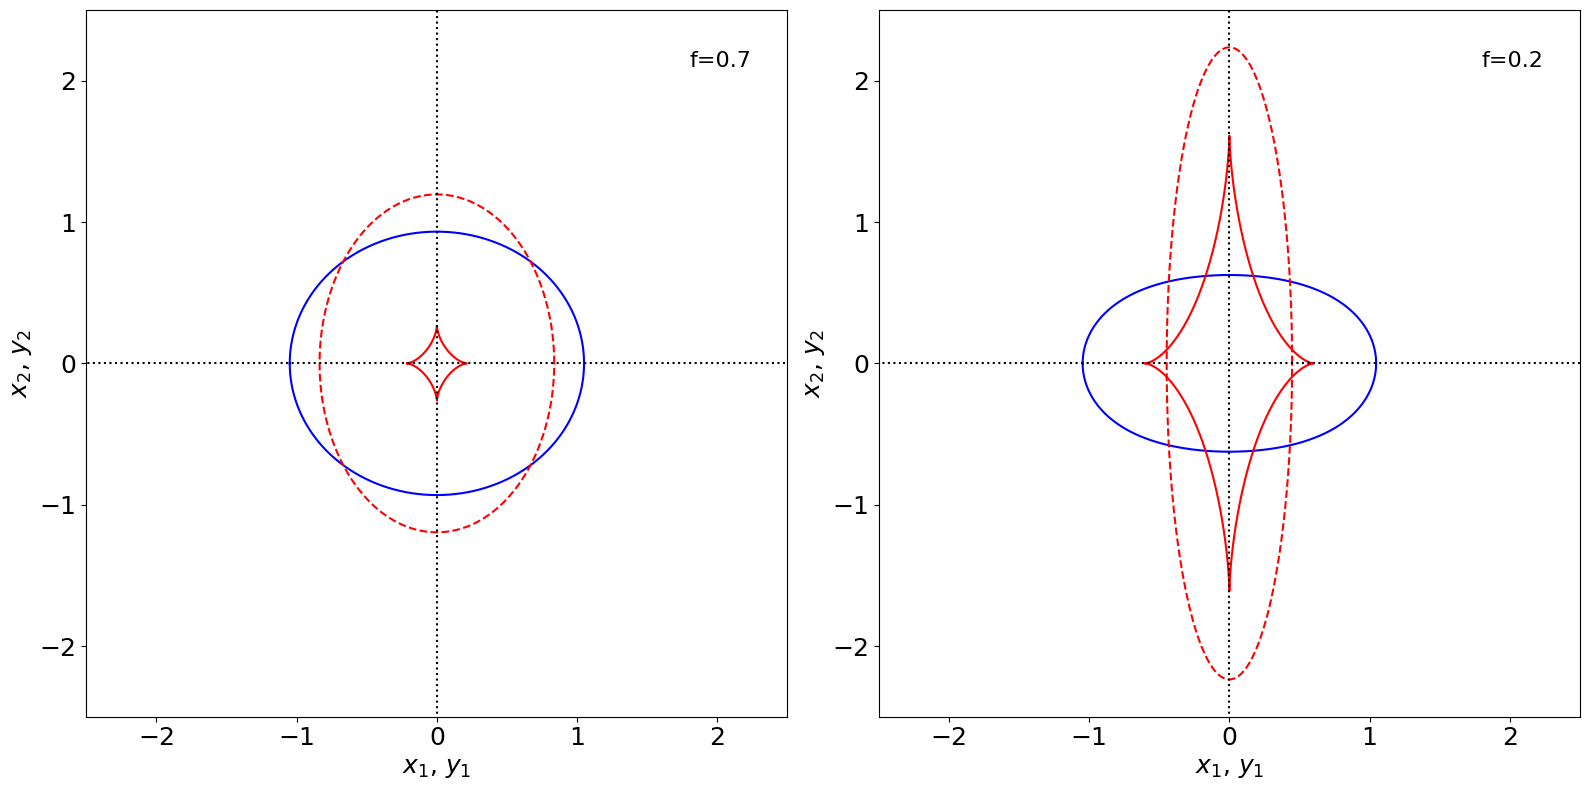
\includegraphics[width=\linewidth, keepaspectratio]{img//chapter3/naked_cusps.png}
    \caption[SIE caustics and critical lines]{Tangential critical line (dashed red), tangential caustic (solid red) and cut (solid blue) for two SIE lenses with $f = 0.7$ and $f = 0.2$.}
    \label{fig:naked_cusps}
\end{figure}

Given that crossing the cut alters the number of images by one and traversing the caustic alters it by two, the scenarios with $f > f_0$ are capable of generating one, two, or four images. In contrast, a smaller value of $f$ can lead to the existence of another possible scenario with the formation of three multiple images (see \cref{fig:sie}).

\begin{figure}
  \begin{minipage}{0.5\linewidth}
    \centering
    \subfloat[]{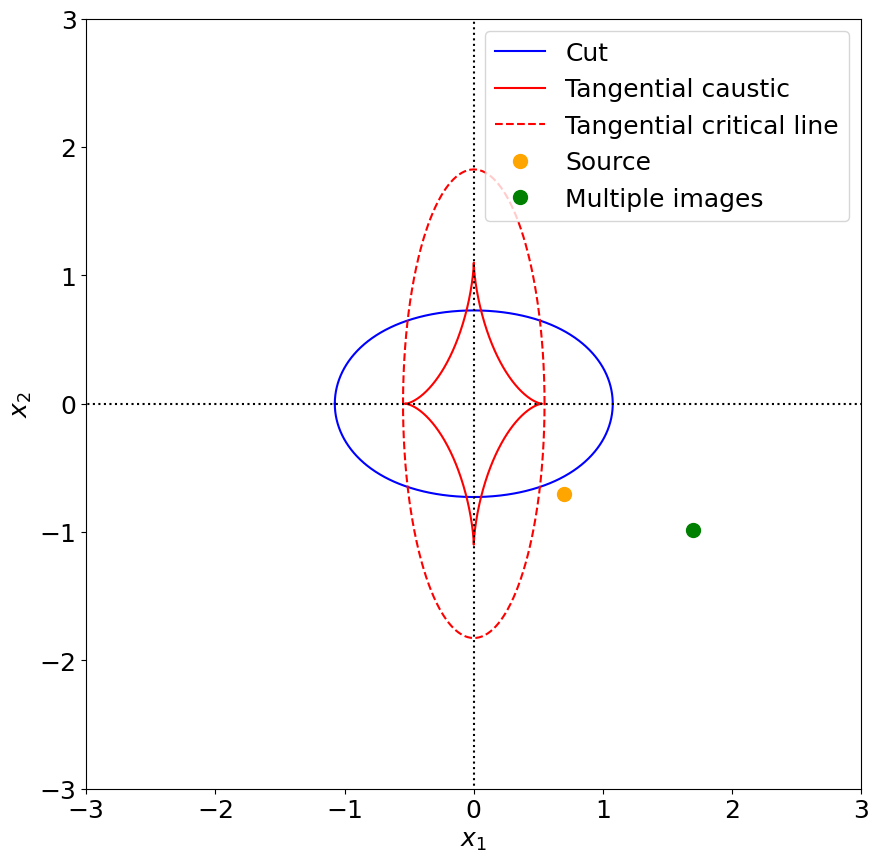
\includegraphics[width=\linewidth, keepaspectratio]{img/chapter3/sie1.png}\label{fig:sie1}}
  \end{minipage}%%
  \begin{minipage}{0.5\linewidth}
    \centering
    \subfloat[]{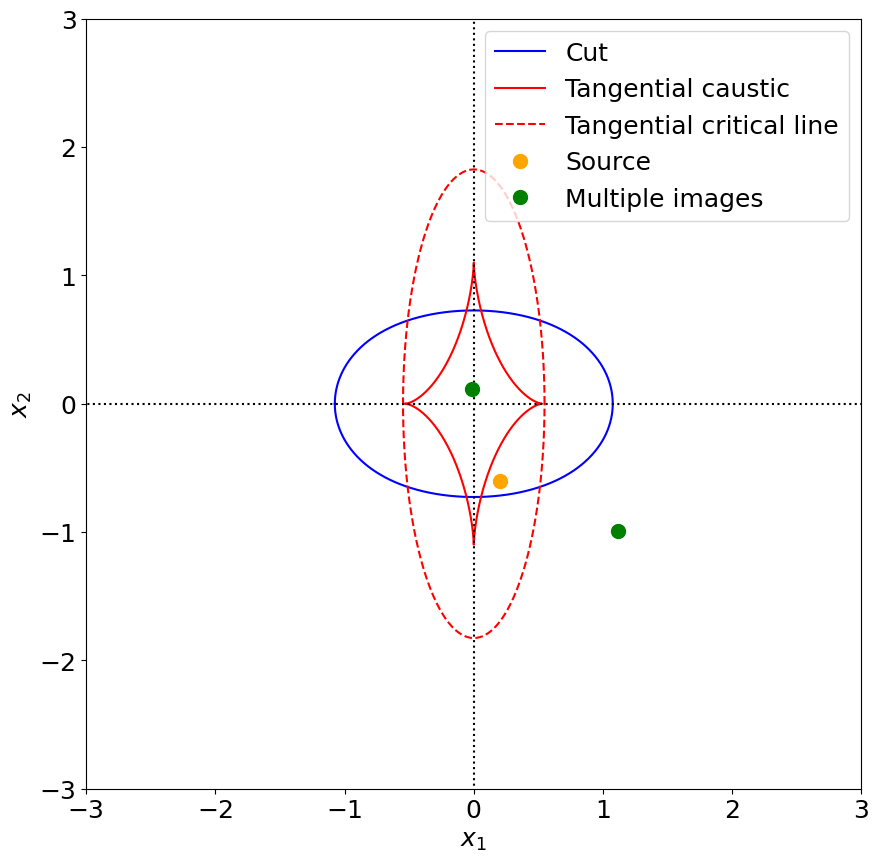
\includegraphics[width=\linewidth, keepaspectratio]{img/chapter3/sie2.png}\label{fig:sie2}}
  \end{minipage} 
  \begin{minipage}{0.5\linewidth}
    \centering
    \subfloat[]{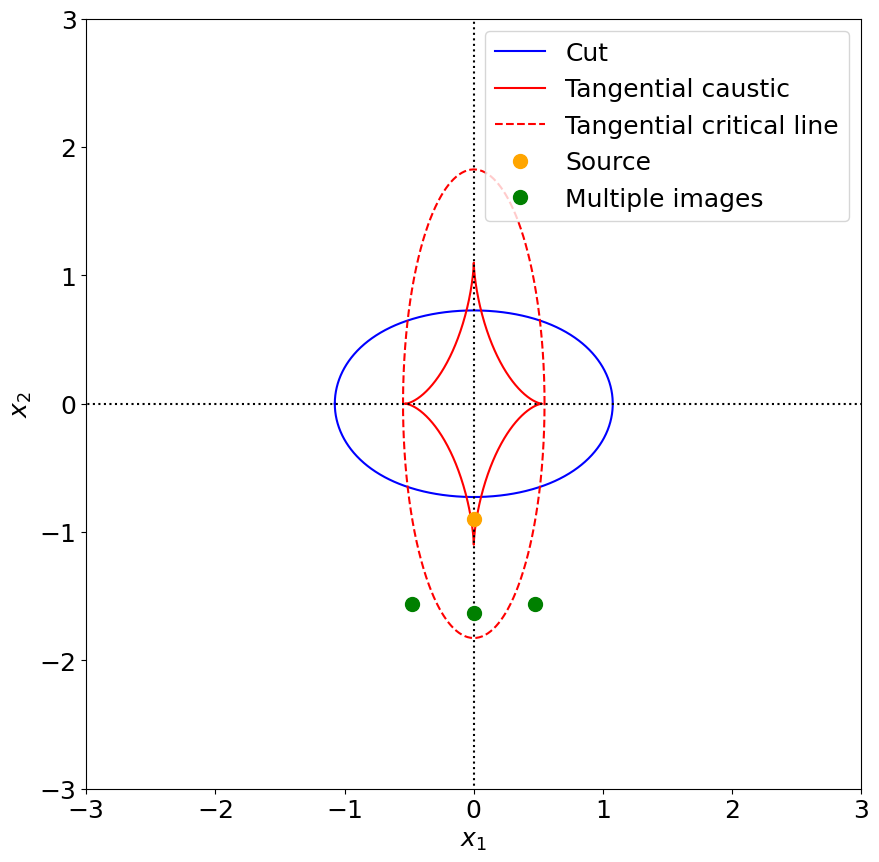
\includegraphics[width=\linewidth, keepaspectratio]{img/chapter3/sie3.png}\label{fig:sie3}}
  \end{minipage}%% 
  \begin{minipage}{0.5\linewidth}
    \centering
    \subfloat[]{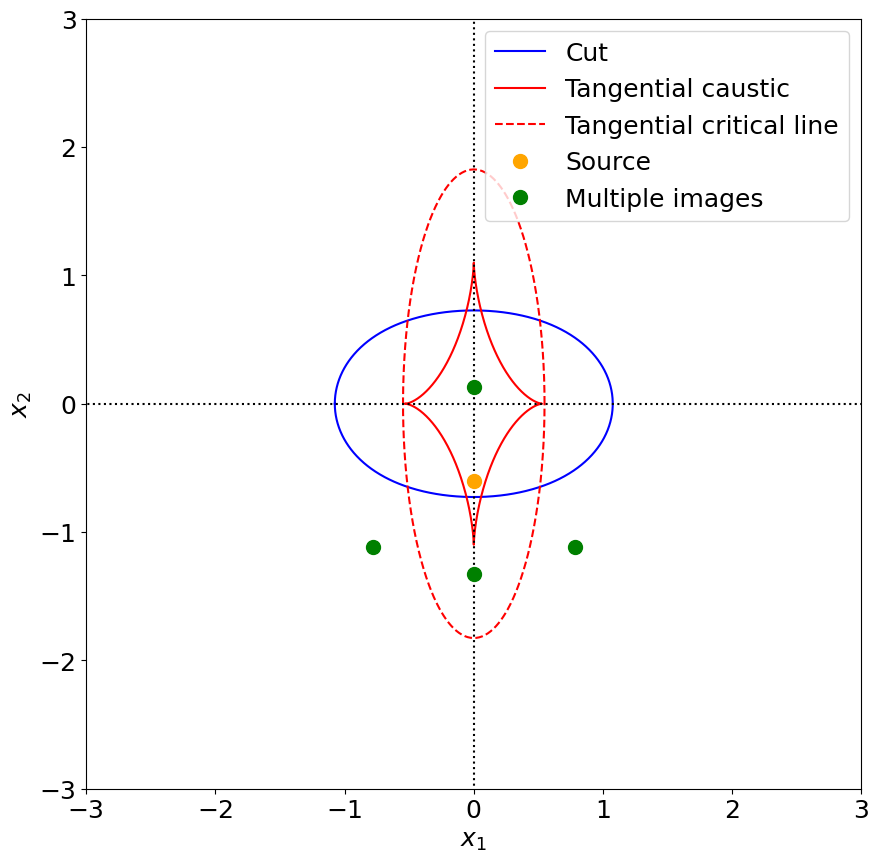
\includegraphics[width=\linewidth, keepaspectratio]{img/chapter3/sie4.png}\label{fig:sie4}}
  \end{minipage} 
  \caption[Image multiplicity for a SIE lens]{Illustration of the different image multiplicity scenarios: \protect\subref{fig:sie1} one image if the source is outside the cut, \protect\subref{fig:sie2} two images if the source is inside the cut, \protect\subref{fig:sie3} three images if the source is inside the caustic and \protect\subref{fig:sie4} four images if the source is inside both caustic and cut.}
  \label{fig:sie}
\end{figure}

\Cref{fig:sie_multiple_images} illustrate the lensing of circular sources by a SIE lens.
The upper panels illustrate the change in image geometry as the source approaches the lens center, traversing the cut and the caustic fold. Sources positioned outside the cut generate a single image, which is located in the same quadrant of the image plane as the source's projected position. Upon crossing the cut, an additional image emerges near the lens center, a consequence directly related to the cut definition. As the source moves nearer to the caustic, the central image shifts away from the lens center, appearing in the quadrant of the lens plane that is opposite to the source's projected quadrant. When the source crosses the caustic, a pair of images appear on either side of the critical line. Specifically, if the source is close to the fold in the source plane's first quadrant, the resultant images are found in the lens plane's second quadrant, adhering to the left-right mapping rule relevant to tangential critical points. As the source approaches the lens center, the resulting images form a symmetrical arrangement known as the \emph{Einstein cross}.

In the middle and bottom panels of \cref{fig:sie}, which focus on the same lens, the source moves from beyond the cut towards the lens's center, crossing through the tangential caustic cusps. At the point of caustic crossing, three images converge at the critical line, with the left-right rule once again coming into effect.

Images near the critical line are distorted tangentially, leading to the creation of \emph{gravitational arcs}. These images become elongated and tend to converge at the critical line, with the most significant gravitational arcs forming from the convergence of three images of sources located near the caustic cusps. The extent of observed distortions is influenced by the source's size in relation to the caustic. When the source is significantly larger than the caustic, the impact of the ellipticity is barely noticeable.

\begin{figure}
    \centering
    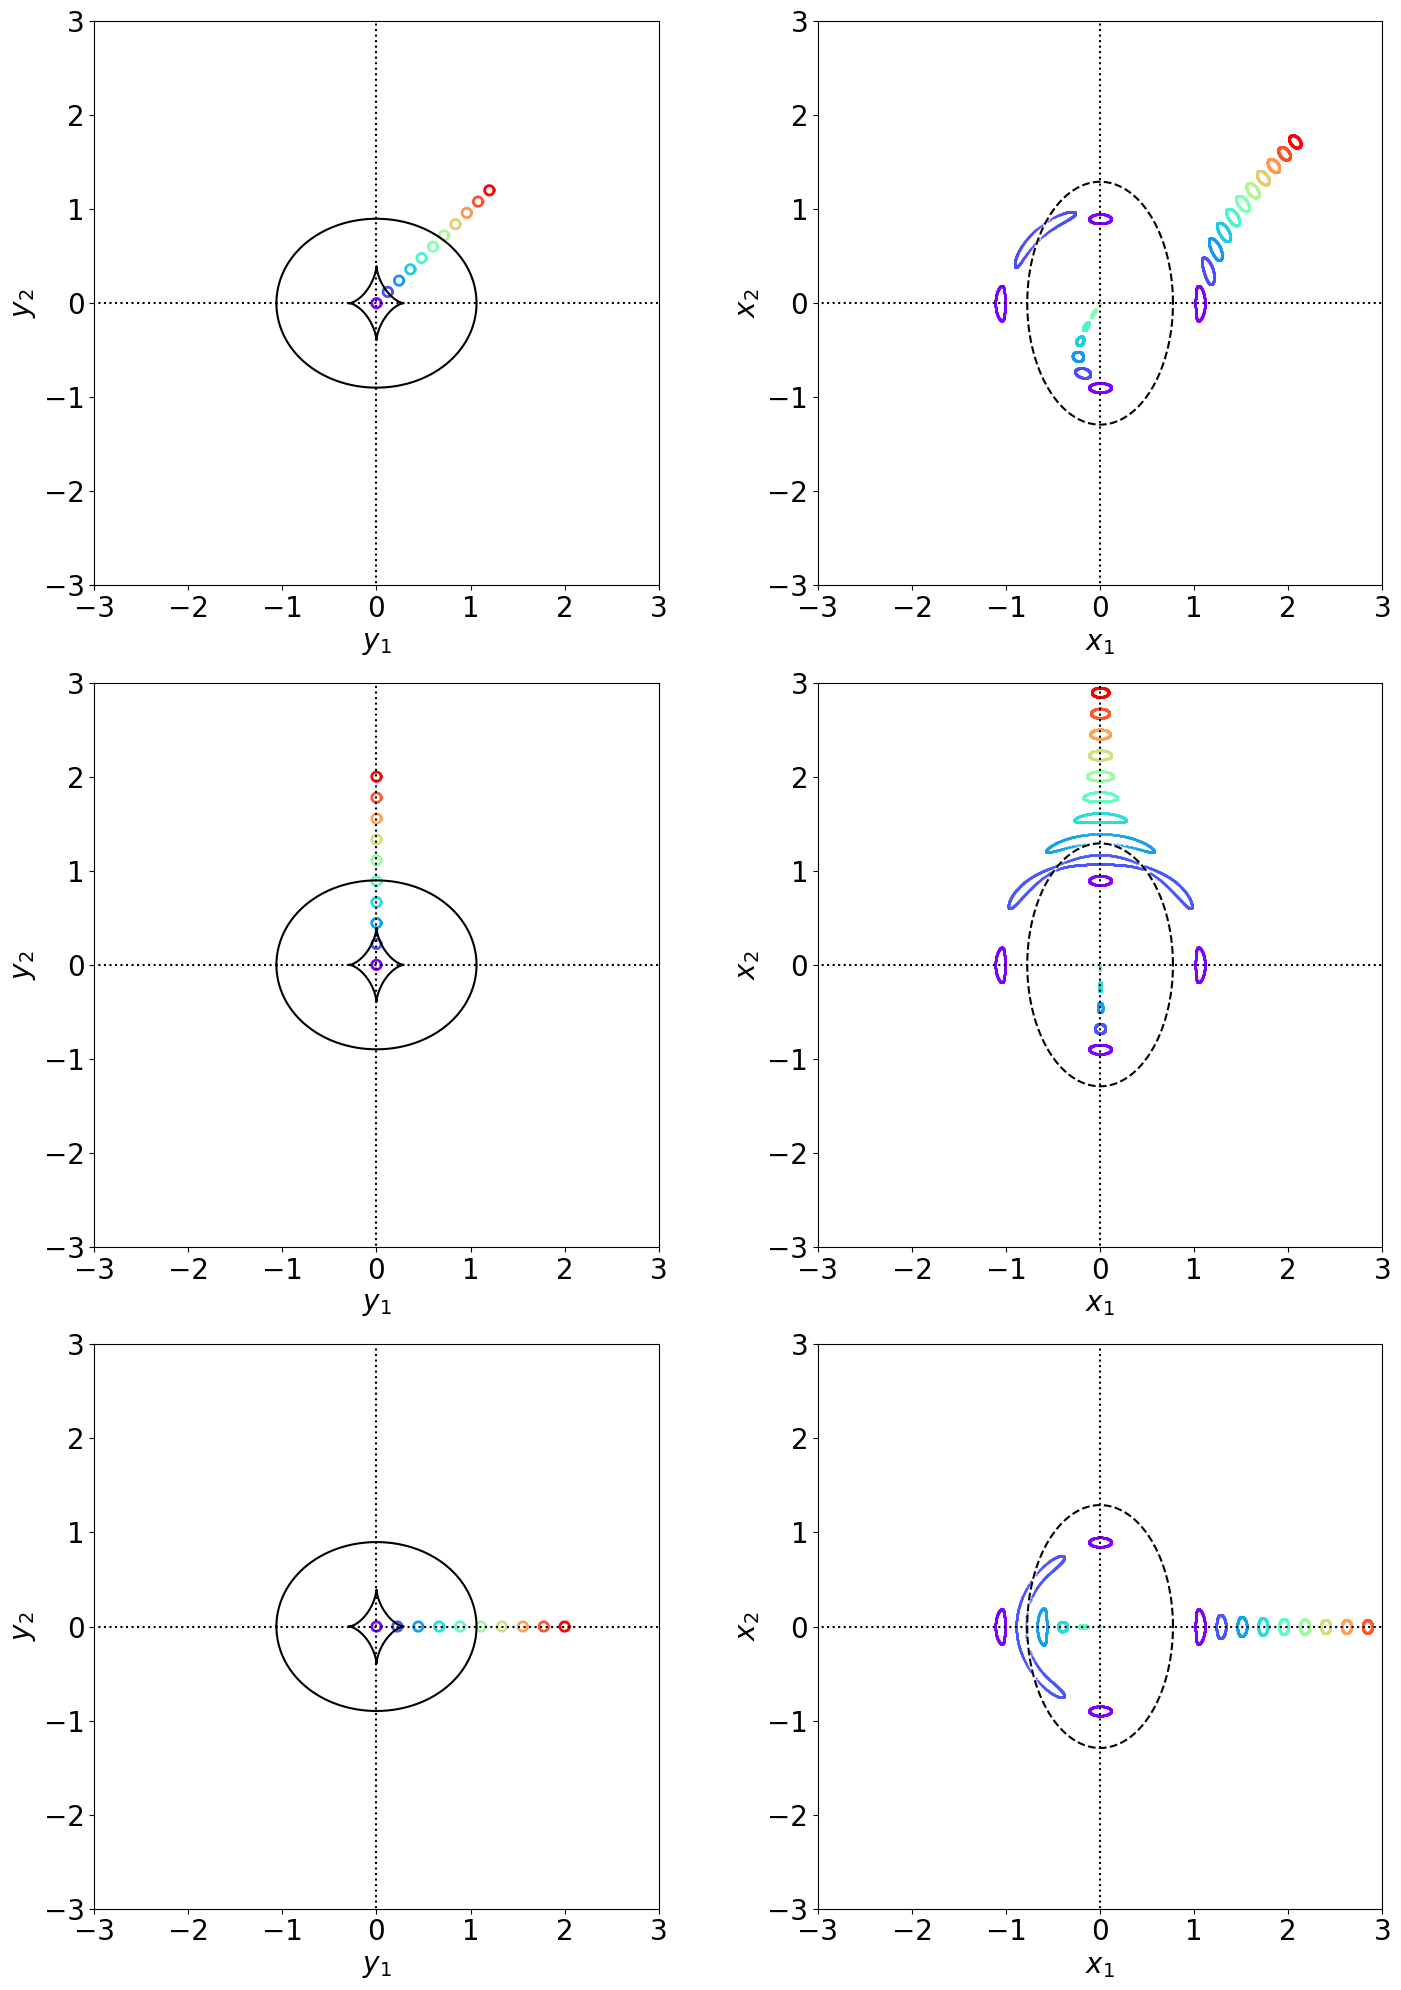
\includegraphics[width=0.9\linewidth, keepaspectratio]{img//chapter3/sie_multiple_images.png}
    \caption[Lensing of circular sources by a SIE]{Lensing of circular sources by a SIE lens with $f=0.6$. In the left panels, sources at different angular separations from the lens center. In the right panels, the correspondent multiple images.}
    \label{fig:sie_multiple_images}
\end{figure}


%%%%%%%%%%%%%%%%%%%%%%%%%%%%%%%%%%%%%%%%%%%%%%%%%%%%%%%
%%%%% Non-singular Isothermal Ellipsoid %%%%%
%%%%%%%%%%%%%%%%%%%%%%%%%%%%%%%%%%%%%%%%%%%%%%%%%%%%%%%
\subsection{Non-singular Isothermal Ellipsoid}
\label{subsec:nie}
As previously done with the SIS model, to remove the central singularity of the surface mass density, it is also possible to introduce a core for the SIE model. The resulting model, the Non-singular Isothermal Ellipsoid (NIE), has been thoroughly described by \cite{kormann_isothermal_1994,tessore_elliptical_2015}. By introducing a core radius $\x_c$ and with the usual choice of $\x_0 = \x_{0,SIS}$, the surface mass density and the convergence can be written
\begin{subequations}
\begin{align}
    \label{eq:3.42a}
    \S (\va{\x}) & = \frac{\s^2}{2 G} \frac{\sqrt{f}}{\sqrt{\x_1^2 + f^2 \x_2^2 + \x_c^2}} \,,
    \\
    \label{eq:3.42b}
    \k (\vec{x}) & = \frac{\sqrt{f}}{2 \sqrt{x_1^2 + f^2 x_2^2 + x_c^2}} \,.
\end{align}
\end{subequations}

\Cref{fig:nie} shows the different multiplicities that a NIE lens can produce of a source, depending on the value of $f$ and $x_c$. It can have two separate critical lines and caustics, only one tangential critical line and caustic, or no critical lines and caustics at all. Depending on the caustics structure, this lens can produce one, three, or five images of a source.

\begin{figure}[b!]
    \centering
    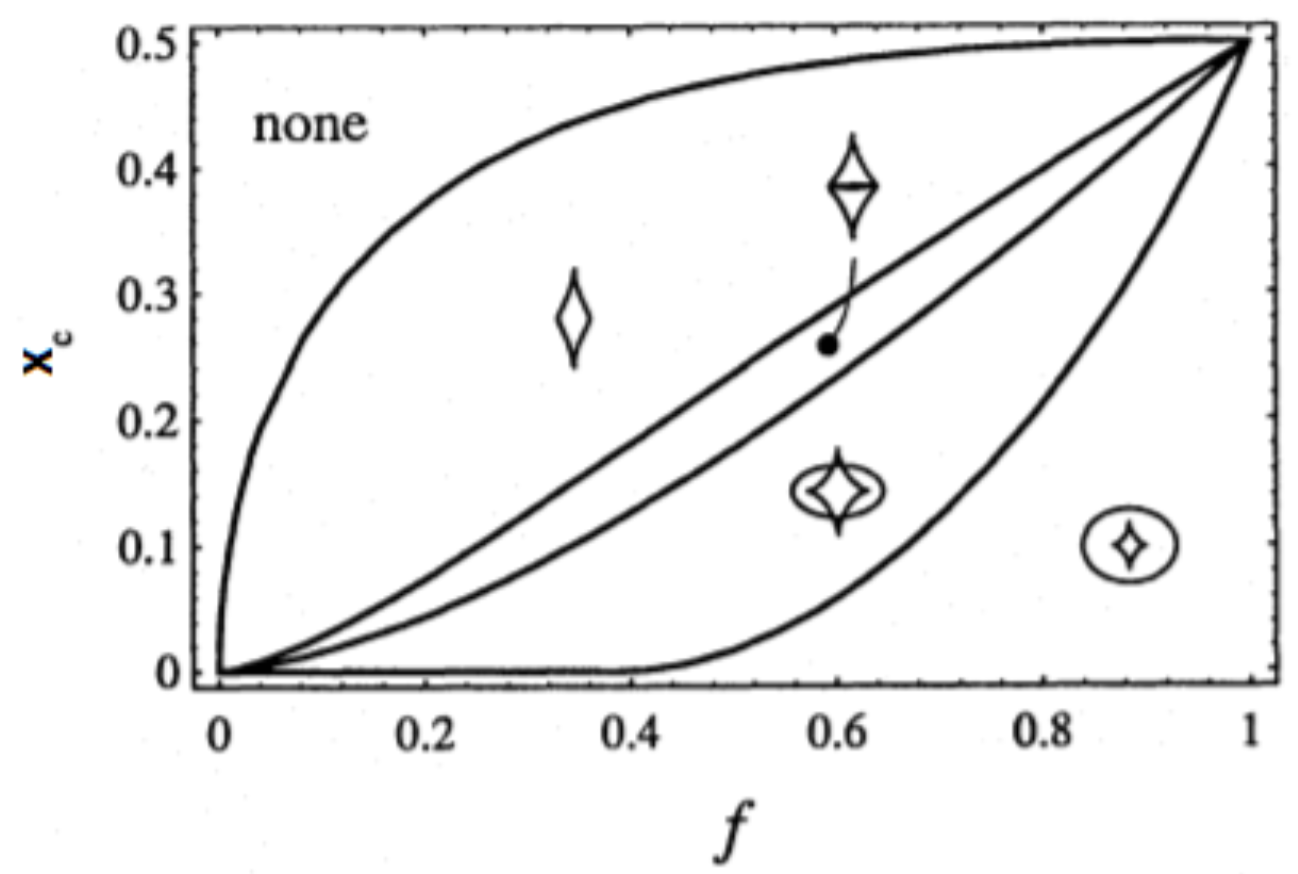
\includegraphics[width=0.9\linewidth]{img//chapter3/nie.png}
    \caption[NIE caustics topologies]{NIE caustics topologies for varying $f$ and $x_c$.\\\small{Credits: \cite{kormann_isothermal_1994}.}}
    \label{fig:nie}
\end{figure}


%%%%%%%%%%%%%%%%%%%%%%%%%%%%%%%%%%%%%%%%%%%%%%%%%%%%%%%
%%%%% External shear %%%%%
%%%%%%%%%%%%%%%%%%%%%%%%%%%%%%%%%%%%%%%%%%%%%%%%%%%%%%%
\subsection{External shear}
\label{subsec:ext_shear}
When analyzing a gravitational lens located in a densely populated environment, it becomes crucial to consider the gravitational influence of the surrounding mass distributions. A usual approach to encapsulate the effects of this environment is to employ the concept of an external shear field. This field is characterized through a potential that allows the quantification of the environmental impact on the lensing effects observed. The external shear field effectively models the tidal forces exerted by nearby mass distributions that are not directly part of the lens, but nevertheless influence the path of light rays passing near the lens.

The presence of the external shear field can be modeled by means of a potential $\P_\g$, such that
\begin{equation}
\begin{aligned}
    \label{eq:3.43}
    \g_1 & = \frac{1}{2} (\P_{11} - \P_{22}) = \mathrm{const.}
    \\
    \g_2 & = \P_{12} = \mathrm{const.}
    \\
    \k & = \frac{1}{2} (\P_{11} + \P_{22}) = \mathrm{const.}
\end{aligned}
\end{equation}

This means that $\P_{11}$ and $\P_{22}$ must be both constants and the potential is quadratic:
\be
\label{eq:3.44}
\P_\g (\vec{x}) = C x_1^2 + C^\prime x_2^2 + D x_1 x_2 + E \,.
\ee

Differentiating \cref{eq:3.44} and substituting into \cref{eq:3.43}:
\begin{equation}
\begin{aligned}
    \label{eq:3.45}
    \g_1 & = \frac{1}{2} (\P_{11} - \P_{22}) = C - C^\prime \,,
    \\
    \g_2 & = \P_{12} = D \,,
    \\
    \k & = \frac{1}{2} (\P_{11} + \P_{22}) = C + C^\prime \,.
\end{aligned}
\end{equation}

At this point, it is possible to distinguish two cases:
\begin{itemize}
    \item $\k = 0$ if the external perturbation does not contribute to the convergence, which means $C = C^\prime = \g_1 / 2$ and
    \be
    \label{eq:3.46}
    \P_\g = \frac{\g_1}{2} (x_1^2 - x_2^2) + \g_2 x_1 x_2 \,.
    \ee
    \item $\g_1, \g_2 = 0$ if the lens is embedded in a sheet of constant surface mass density producing no shear (no privileged directions); in this case the external convergence potential is
    \be
    \label{eq:3.47}
    \P_\k = \frac{\k}{2} x^2 \,,
    \ee
    and can be inserted into the lens equation
    \be
    \label{eq:3.48}
    \va{\a} (\vec{x}) = \va{\nabla} \P_\k (\vec{x}) = \k \vec{x} \,,
    \ee
    to obtain
    \be
    \label{eq:3.49}
    \vec{y} = \vec{x} - \va{\a} (\vec{x}) = \vec{x} (1 - \k) \,.
    \ee

    If $\k = 1$, this sheet acts as a perfectly convergent lens, mapping every position $\vec{x}$ on the lens plane to the same point $y=0$.
\end{itemize}